%%%%%%%%%%%%%%%%%%%%%%%%%%%%%%%%%%%%%%%%%%%%%%%%%%%%%%%%%%%%%%%%%%%%%%%%%%%
%% This file is part of the book
%%
%% Algorithmic Graph Theory
%% http://code.google.com/p/graph-theory-algorithms-book/
%%
%% Copyright (C) 2009--2011 Minh Van Nguyen <nguyenminh2@gmail.com>
%%
%% See the file COPYING for copying conditions.
%%%%%%%%%%%%%%%%%%%%%%%%%%%%%%%%%%%%%%%%%%%%%%%%%%%%%%%%%%%%%%%%%%%%%%%%%%%

\documentclass{article}

\usepackage{subfigure}
\usepackage{tikz}
\usetikzlibrary{external}
\tikzexternalize{search-Petersen-graph}

\begin{document}

\begin{figure}
%% breadth-first searching the Petersen graph
\subfigure[Breadth-first search.]{
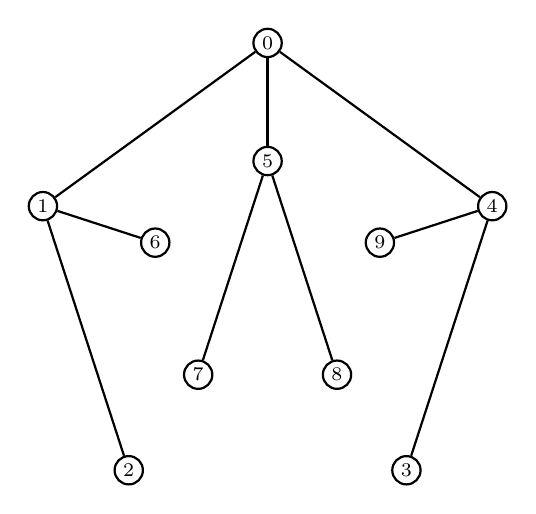
\begin{tikzpicture}
[lineDecorate/.style={-,thick},%
  nodeDecorate/.style={shape=circle,inner sep=1.5pt,draw,thick},%
  scale=1.5]
%% nodes or vertices
\foreach \nodename/\x/\y in {
  %% inner star
  5/0.0/1.0, 9/0.9510/0.3090, 8/0.5877/-0.8090, 7/-0.5877/-0.8090,
  6/-0.9510/0.3090,
  %% outer pentagon
  0/0.0/2.0, 4/1.9021/0.6180, 3/1.1755/-1.6180, 2/-1.1755/-1.6180,
  1/-1.9021/0.6180}
{
  \node (\nodename) at (\x,\y) [nodeDecorate] {\scriptsize$\nodename$};
}
%% edges or lines
\path
\foreach \startnode/\endnode in {
  0/1, 0/4, 0/5, 1/2, 1/6, 4/3, 4/9, 5/7, 5/8}
{
  (\startnode) edge[lineDecorate] node {} (\endnode)
};
\end{tikzpicture}
}
\qquad
%%
%%
%% depth-first searching the Petersen graph
\subfigure[Depth-first search.]{
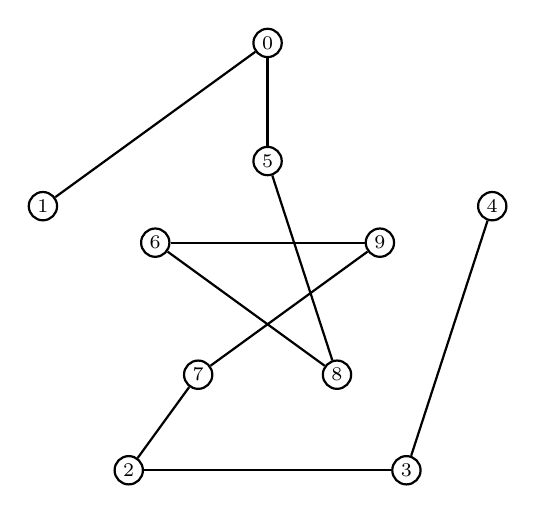
\begin{tikzpicture}
[lineDecorate/.style={-,thick},%
  nodeDecorate/.style={shape=circle,inner sep=1.5pt,draw,thick},%
  scale=1.5]
%% nodes or vertices
\foreach \nodename/\x/\y in {
  %% inner star
  5/0.0/1.0, 9/0.9510/0.3090, 8/0.5877/-0.8090, 7/-0.5877/-0.8090,
  6/-0.9510/0.3090,
  %% outer pentagon
  0/0.0/2.0, 4/1.9021/0.6180, 3/1.1755/-1.6180, 2/-1.1755/-1.6180,
  1/-1.9021/0.6180}
{
  \node (\nodename) at (\x,\y) [nodeDecorate] {\scriptsize$\nodename$};
}
%% edges or lines
\path
\foreach \startnode/\endnode in {
  0/5, 5/8, 8/6, 6/9, 9/7, 7/2, 2/3, 3/4, 0/1}
{
  (\startnode) edge[lineDecorate] node {} (\endnode)
};
\end{tikzpicture}
}
\end{figure}

\end{document}
